\documentclass[10pt, oneside]{article}
\usepackage{amsmath, amsthm, amssymb, calrsfs, wasysym, verbatim, bbm, color, graphics, graphicx, geometry}
\usepackage[most]{tcolorbox}
\usepackage{xcolor}
\usepackage{framed}
\usepackage{ragged2e}
\usepackage{amsmath}
\colorlet{shadecolor}{blue!15}
\graphicspath{ {./} }
\geometry{tmargin=.75in, bmargin=.75in, lmargin=.75in, rmargin=.75in}
\newcommand{\R}{\mathbb{R}}
\newcommand{\C}{\mathbb{C}}
\newcommand{\Z}{\mathbb{Z}}
\newcommand{\N}{\mathbb{N}}
\newcommand{\Q}{\mathbb{Q}}
\newcommand{\Cdot}{\boldsymbol{\cdot}}
\newtheorem{thm}{Theorem}
\newtheorem{defn}{Definition}
\newtheorem{conv}{Convention}
\newtheorem{rem}{Remark}
\newtheorem{lem}{Lemma}
\newtheorem{cor}{Corollary}
\newtheorem{exa}{Example}

\title{Clase \# 5: Dinámica de los fluidos [MF100]}
\author{\textbf{Luis Alejandro Morales}\\ \vspace{0.4cm} Profesor Asistente \\ Universidad Nacional de Colombia-Bogot\'a\\Facultad de Ingenier\'ia \\ Departamento de Ingeniería Civil y Agr\'icola}
\date{Periodo 2024-I}

\begin{document}

\maketitle
\tableofcontents

\vspace{.25in}

\section{Ecuación de energía}
El principio de conservación de la energía establece que la energía neta transferida a un sistema o extraída de él durante un proceso debe ser igual al cambio en el contenido de energía de ese sistema. En los volúmenes de control, la transferencia de energía también puede ocurrir a través del flujo de masa.
En articulación con los temas trabajados, ya hemos encontrado expresiones que trabajan sobre la conservación de la masa sobre un fluido, ahora es importante pensar en que la energía puede ser transferida a un sistema cerrado o extraída de él mediante calor o trabajo.  El principio de conservación de la energía, también conocido como balance de energía, se expresa como:

\begin{equation}
E_{\text{entrada}} - E_{\text{salida}} = \frac{dE_{\text{VC}}}{dt}
\label{patl}
\end{equation}

\begin{figure}[h]
\centering
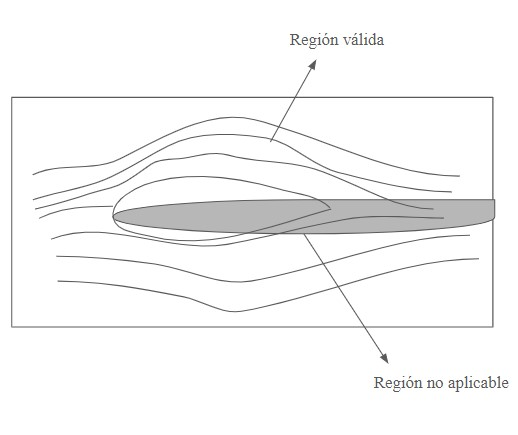
\includegraphics[width=8cm]{Fig.1.jpg}
\caption{Representación de la línea de energía}
\label{eulan}
\end{figure}

\subsection{Ecuación de Bernoulli}
La ecuación de Bernoulli establece una relación simplificada entre la presión, la velocidad y la elevación en regiones de flujo estacionario e incompresible, donde las fuerzas de fricción netas son insignificantes. A pesar de su simplicidad, esta ecuación ha demostrado ser una herramienta poderosa en mecánica de fluidos dada su "aplicabilidad" a varias regiones de un campo de flujo práctico. Estas regiones se denominan  \textbf{regiones de flujo no viscoso}, destacando que no implican la ausencia de viscosidad o fricción en el fluido, sino más bien que las fuerzas viscosas netas son insignificantes en comparación con otras fuerzas que actúan sobre las partículas del fluido.
Para efectos de aproximación se asume que los efectos viscosos son notablemente pequeños en comparación con los efectos de inercia, gravedad y presión. Esto último no es válido en todo el campo de flujo, por ende, la ecuación de Bernoulli no puede aplicarse universalmente en un flujo, independientemente de la baja viscosidad del fluido, por lo general se puede usar en regiones lejanas a las paredes del sistema o a las denominadas \textbf{capas límite}.
Para el análisis es válido mencionar que el movimiento de una partícula y su trayectoria se caracterizan por el vector velocidad, que varía con el tiempo y las coordenadas espaciales, además de la posición inicial de la partícula. En flujos estacionarios, donde no hay cambios temporales en un punto específico, todas las partículas que pasan por el mismo punto siguen una trayectoria constante, conocida como línea de corriente. Esta línea representa la senda que sigue el fluido y en la cual los vectores de velocidad son tangentes en cada punto. La utilidad de este concepto es más evidente en regiones del flujo fuera de las capas límite y estelas, donde predominan los efectos combinados de la presión y la gravedad.

\begin{equation}
P + \frac{1}{2} \rho v^2 + \rho gh = \text{cte}
\end{equation}

Para una sección delimitada por un volumen de control y que es analizada en dos secciones tenemos que la ecuación puede ser reescrita como:
\begin{equation}
P_1 + \frac{1}{2} \rho v_1^2 + \rho g h_1 = P_2 + \frac{1}{2} \rho v_2^2 + \rho g h_2
\end{equation}

El movimiento de una partícula y la trayectoria que sigue se describen mediante el vector velocidad, el cual es una función del tiempo, las coordenadas espaciales y la posición inicial de la partícula. Cuando el flujo es estacionario (sin cambios con el tiempo en un lugar específico), todas las partículas que pasan por el mismo punto siguen la misma trayectoria (que es la línea de corriente) y los vectores de velocidad permanecen tangentes a la trayectoria en todo punto.
 
\subsection*{Principio de Conservación de la Energía}
Dado el principio de conservación de la energía, se establece que la suma de los cambios en la energía cinética y potencial debe ser igual al trabajo realizado por la presión:
$$ 
P \, dV + \frac{1}{2} \, \rho \, dV \, dv^2 + \rho \, g \, dV \, dh = 0
$$

Dividiendo todo por \(dV\) y reorganizando términos, obtenemos:
$$
P + \frac{1}{2} \rho v^2 + \rho g h = \text{cte}
$$

\subsection{Línea de energía y de gradiente hidráulico}
Teniendo claridad en cada parte que compone la ecuación de Bernoulli, es conveniente representar de manera gráfica el nivel de la energía mecánica, usando alturas, con la finalidad de facilitar la visualización de los diversos términos de la ecuación de Bernoulli. Esto se puede realizar dividiendo
cada término de esa ecuación entre el valor de la gravedad (g), obteniendo:

\begin{equation}
\frac{P_1}{\rho g} + \frac{v_1^2}{2g} + h_1 = \text{H} = \text{cte}
\label{ace}
\end{equation}

Cada término de esta ecuación hace referencia a una carga de fluido fluyente con sus respectivas dimensiones y longitud:

\begin{itemize}
    \item $\frac{P_1}{\rho g}$ representa la carga por presión equivalente a la columna de fluido que produce la presión estática.
    \item $\frac{v_1^2}{2g}$ corresponde a la cabeza de velocidad del fluido y representa la elevación que se necesita para que dicho fluido alcance la velocidad \(v\) en caída libre y despreciando la fricción.
    \item Finalmente, $h_1$ corresponde a la cabeza de elevación del fluido y nos indica su energía potencial.
\end{itemize}

Del mismo modo, \( H \) representa la carga total del flujo, que es la suma de las cargas de presión, de velocidad y de elevación a lo largo de una línea de corriente. Esta suma es constante durante el flujo estacionario, bajo las condiciones en las que la ecuación de Bernoulli es aplicable.

Por ejemplo, si se coloca un piezómetro (que mide la presión estática) en una toma en un tubo, el líquido subirá hasta una altura de \( \frac{P}{\rho g} \) por encima del centro del tubo. La línea de gradiente hidráulico (LGH), también conocida como línea piezométrica o línea de alturas piezométricas, se obtiene al realizar esta medición en varios puntos a lo largo del tubo y trazar una línea que conecte los niveles del líquido en los piezómetros.

% Fig 4-8 Cengel 
\begin{figure}[h]
\centering
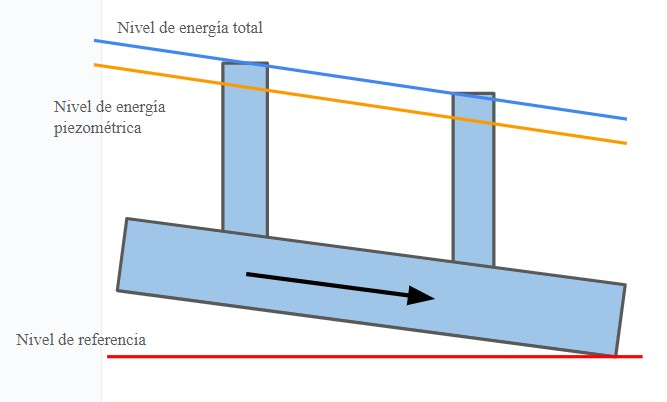
\includegraphics[width=8cm]{Fig.2.jpg}
\caption{Representación de nivel de energía y nivel ´piezométrico (LGH)}
\label{acel}
\end{figure}

\subsection{Aceleración en una partícula}
La aceleración de una partícula de fluido se describe frecuentemente en términos de su distancia \( s \) a lo largo de una línea de corriente y su radio de curvatura a lo largo de esta línea. En flujos bidimensionales, la aceleración se posee dos componentes: la aceleración tangencial \( a_s \), a lo largo de la línea de corriente, y la aceleración normal \( a_n \), en la dirección perpendicular a la línea.
La aceleración tangencial \( a_s \) se debe a cambios en la magnitud de la velocidad a lo largo de la línea de corriente, mientras que la aceleración normal \( a_n \) se debe a cambios en la dirección de la velocidad, expresada como \( \frac{V^2}{R} \) a lo largo de una trayectoria curva, donde \( R \) es el radio de curvatura. En el caso de partículas que se mueven a lo largo de una línea recta, la aceleración normal es cero, ya que el radio de curvatura es infinito y no hay cambio en la dirección de la velocidad.
\begin{equation}
\frac{dV}{dt} = \frac{\partial V}{\partial t}\frac{ds}{dt} + \frac{\partial V}{\partial t}
\end{equation}
 Considerando el flujo estacionario: 
 \begin{equation}
   a_s = V \frac{\partial V}{\partial s}  
 \end{equation}
 
La ecuación de Bernoulli surge de un balance de fuerzas a lo largo de una línea de corriente. Es importante no confundir el concepto de flujo estacionario con la ausencia de aceleración. Aunque en un flujo estacionario no hay cambio en el tiempo en un punto fijo, puede haber cambios en la velocidad y en la aceleración a lo largo de la trayectoria del fluido. Por ejemplo, en el caso de una boquilla de una manguera de jardín, el flujo de agua se acelera a medida que pasa por la boquilla, a pesar de que el flujo de masa sea constante. Esto ilustra que "estacionario" simplemente significa que no hay cambio temporal en un punto fijo, pero las propiedades del flujo pueden variar de un punto a otro.


\begin{figure}[h]
\centering
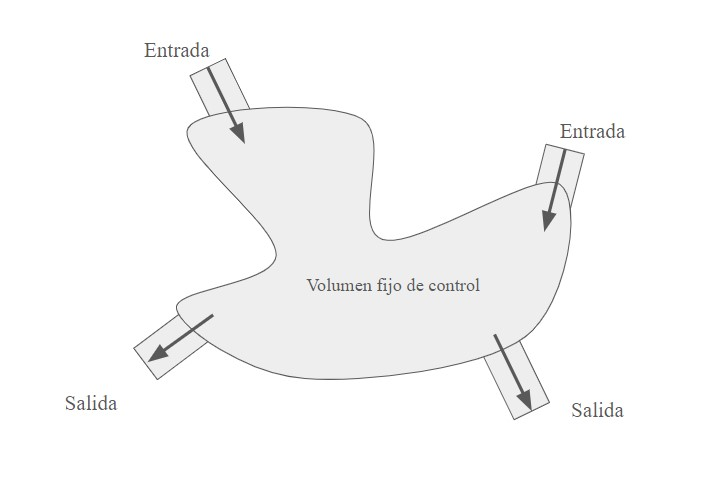
\includegraphics[width=8cm]{Fig.3.jpg}
\caption{Sistema con múltiples entradas y salidas}
\label{eulan}
\end{figure}
\subsection{Potencia hidráulica}

La potencia hidráulica \( P \) se define como la tasa de trabajo realizado por el fluido en un sistema hidráulico. Para un fluido incompresible y estacionario, la potencia se puede expresar de varias formas, dependiendo de la aplicación específica:

\begin{itemize}
    \item \textbf{Potencia por unidad de masa:}
    $$
    \dot{P} = \dot{m} \left( h_1 + \frac{v_1^2}{2} + gz_1 - h_2 - \frac{v_2^2}{2} - gz_2 \right)
    $$
    donde:
    \begin{itemize}
        \item \( \dot{m} \) es el flujo másico del fluido,
        \item \( h \) es la altura de la carga de presión,
        \item \( v \) es la velocidad del fluido,
        \item \( g \) es la aceleración debido a la gravedad,
        \item \( z \) es la altura sobre un nivel de referencia.
    \end{itemize}
    
    \item \textbf{Potencia por unidad de volumen:}
    $$
    P = \rho \dot{V} \left( h_1 + \frac{v_1^2}{2} + gz_1 - h_2 - \frac{v_2^2}{2} - gz_2 \right)
    $$
    donde:
    \begin{itemize}
        \item \( \rho \) es la densidad del fluido,
        \item \( \dot{V} \) es el flujo volumétrico del fluido.
    \end{itemize}
\end{itemize}

Estas expresiones representan la potencia hidráulica en términos de la diferencia de energía entre dos puntos del flujo, teniendo en cuenta las contribuciones de la presión, la velocidad y la elevación del fluido.

\section{Conservación de momentum}

El concepto de cantidad de momento lineal se basa en las leyes fundamentales de Newton, las cuales describen las relaciones entre los movimientos de los cuerpos y las fuerzas que actúan sobre ellos.
La segunda Ley de Newton relaciona la aceleración de un cuerpo con la fuerza neta que actúa sobre él, expresando que la aceleración es directamente proporcional a la fuerza neta e inversamente proporcional a la masa del cuerpo. Esta ley es fundamental para entender cómo las fuerzas impulsan el movimiento y la dinámica de los fluidos en diferentes condiciones, la misma puede ser escrita como: 

 \begin{equation}
\vec{F} = m \vec{a}  = m \frac{d\vec{V}}{dt} 
 \end{equation}
 
El momento lineal o cantidad de movimiento de un cuerpo se define como el producto de su masa y su velocidad. Para un cuerpo rígido de masa \( m \) moviéndose con una velocidad \( \vec{V} \), su momento lineal se representa como \( m \vec{V} \). Este enfoque es más alineado con el enunciado original de Newton para la segunda ley y es particularmente relevante en la mecánica de fluidos al estudiar las fuerzas resultantes de los cambios de velocidad en los flujos. Por lo tanto, en este campo, es común referirse a la segunda ley de Newton como la \textbf{ecuación del momento lineal}.\\

La cantidad de movimiento de un sistema permanece constante cuando la fuerza neta que actúa sobre él es cero, lo que implica que la cantidad de movimiento de dichos sistemas se conserva. Esto se conoce como el principio de conservación de la cantidad de movimiento. También es necesario destacar que la fuerza, la aceleración, la velocidad y la cantidad de movimiento son magnitudes vectoriales y, como tales, tienen tanto dirección como magnitud.

\subsection{Conservación de momento angular}

Cuando se estudian cuerpos que rotan o sistemas de flujo con movimiento angular. La contraparte de la segunda Ley de Newton para los cuerpos rígidos en rotación se expresa como \( \vec{M} = I \vec{a} \), donde \( \vec{M} \) es el momento o momento de torsión neto aplicado sobre el cuerpo, \( I \) es el momento de inercia respecto al eje de rotación, y \( \vec{a} \) es la aceleración angular.

Esto también puede expresarse en términos de la razón de cambio del momento angular \( \frac{d\vec{H}}{dt} \), donde \( \vec{H} \) es el momento angular, como:

\begin{equation}
\vec{M} = \frac{d\vec{H}}{dt}  = \frac{d(I\vec{w})}{dt} 
\end{equation}

Esta ecuación relaciona el momento aplicado \( \vec{M} \) con la tasa de cambio del momento angular \( \vec{H} \), proporcionando un marco para analizar cómo se transmiten y transforman las fuerzas rotacionales en sistemas de flujo.

\subsection{Ecuación de momento lineal}
A las consideraciones anteriores se añade que tanto la densidad como la velocidad pueden variar de un punto a otro dentro del sistema, la segunda ley de Newton puede expresarse de manera más general como:

\begin{equation}
\sum \vec{F} = \frac{d}{dt} \int \rho \vec{V} \, dV
\end{equation}

Por lo tanto, la segunda ley de Newton puede enunciarse como la suma de todas las fuerzas externas que actúan sobre un sistema, igual a la razón de cambio temporal del momento lineal de ese sistema. Este enunciado es válido para un sistema de coordenadas que está en reposo o se mueve con velocidad constante, conocido como sistema inercial de coordenadas o marco inercial de referencia. Sin embargo, para sistemas en aceleración, como los aviones durante el despegue, es más apropiado utilizar sistemas de coordenadas no inerciales (o en aceleración), fijos al avión, para un análisis más preciso. Si a esto sumamos el RTT tenemos la ecuación general para un volumen de control fijo, móvil o en deformación: 

\begin{equation}
\sum \vec{F}=\frac{d}{d t} \int_{\mathrm{VC}} \rho \vec{V} d V+\int_{\mathrm{SC}} \rho \vec{V}\left(\vec{V}_r \cdot \vec{n}\right) d A
\end{equation}

Esto último se puede condensar en que suma de todas las fuerzas externas de un volumen de control es igual a la razón de cambio de momento lineal en el tiempo, más el flujo neto que sale del volumen de control. 

\subsection{Casos especiales asociados al volumen de control}

La expresión anterior es precisa para volúmenes de control fijos, pero puede resultar poco práctica en la ingeniería debido al uso de integrales, por ello es preferible reformular la expresión en términos de velocidades promedio y flujos de masa a través de entradas y salidas. En numerosas aplicaciones prácticas, el fluido atraviesa las fronteras del volumen de control mediante una o más entradas y salidas, transportando consigo cantidad de movimiento hacia adentro o hacia afuera de dicho volumen.

\subsubsection{Flujo estacionario en reposo}
\begin{equation}
\sum \vec{F}=\sum_{\text {sal }} \beta \dot{m} \vec{V}-\sum_{\mathrm{cnt}} \beta \dot{m} \vec{V}
\end{equation}

La expresión indica que la fuerza neta actuante sobre el volumen de control durante el flujo estacionario en reposo es equivalente a la diferencia entre las tasas de flujo de cantidad de movimiento entrante y saliente.

\subsubsection{Flujo estacionario en reposo: una entrada y una salida}
\begin{equation}
\sum \vec{F}=\dot{m}\left(\beta_2 \vec{V}_2-\beta_1 \vec{V}_1\right)
\end{equation}

Se subraya nuevamente que todas las relaciones mencionadas anteriormente son ecuaciones vectoriales, donde todas las adiciones y sustracciones son vectoriales. Es importante recordar que restar un vector es equivalente a sumarlo después de invertir su dirección. Además, al escribir la ecuación de la cantidad de movimiento a lo largo de una coordenada específica (como el eje x), se utilizan las proyecciones de los vectores sobre dicho eje.

\begin{figure}[h]
\centering
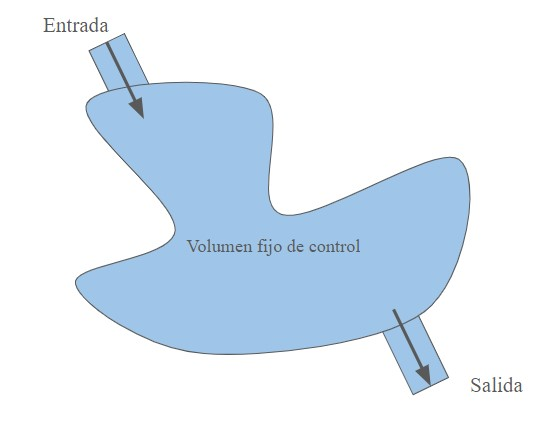
\includegraphics[width=8cm]{Fig.4.jpg}
\caption{Sistema con una entrada y una salida}
\label{eulan}
\end{figure}

\subsubsection{Flujo sin fuerzas externas}
\begin{equation}
0=\frac{d(m \vec{V})_{\mathrm{VC}}}{d t}+\sum_{\mathrm{sal}} \beta \dot{m} \vec{V}-\sum_{\mathrm{ent}} \beta \dot{m} \vec{V}
\end{equation}

Esta es una formulación del principio de conservación de la cantidad de movimiento, que puede enunciarse como: en ausencia de fuerzas externas, la tasa de cambio de la cantidad de movimiento de un volumen de control es igual a la diferencia entre las tasas de flujo de cantidad de movimiento que entran y salen.

\end{document}

